
%(BEGIN_QUESTION)
% Copyright 2006, Tony R. Kuphaldt, released under the Creative Commons Attribution License (v 1.0)
% This means you may do almost anything with this work of mine, so long as you give me proper credit

A control valve (all by itself!) may act as a crude proportional controller for controlling pressure of a gas or vapor:

$$\includegraphics[width=15.5cm]{i01483x01.eps}$$

Identify how this constitutes a negative feedback system, and explain how it works to regulate downstream pressure.  Then, identify what things you would have to change in this system to alter its gain (proportional band) and setpoint.

\underbar{file i01483}
%(END_QUESTION)





%(BEGIN_ANSWER)

The principle is fairly straightforward to figure out, but gain and setpoint are not as easy.  To change gain, you could substitute a different-sized diaphragm in the valve actuator.  Setpoint adjustments could be made by changing the {\it bench set} of the valve.

%(END_ANSWER)





%(BEGIN_NOTES)

One could also alter gain by changing the spring in the actuator assembly with one having a different spring rate (the $k$ factor, as in Hooke's Law: $F = -kx$).

%INDEX% Control, proportional: control valve as crude proportional pressure controller

%(END_NOTES)


